% ============================================================ Capítulo: biblioteca de máquinas (Anatomy)
\chapter{Versión 2.0: biblioteca de máquinas interactivas}\label{cap:anatomia}

\section{Propósito}
La biblioteca es un menú de máquinas interactivas que explican procesos de una planta de autopartes. Cada tarjeta
proporciona información obtenida con el web scraping: la API \texttt{/api/v1/maquinas} busca en la base Gold
(BM25) la oración más pertinente para cada máquina y la entrega con su URL, su identificador de fragmento y su
origen (\texttt{scraping}, \texttt{lectura\_web} o \texttt{semilla}). Los parámetros que mueven la máquina se toman
de la base cuando existen ---por ejemplo, la capacidad de 24\,000 chasises al año de la planta de Bogotá--- y, si
no, se marcan como \texttt{demostrativo}.

\begin{figure}[H]\centering
\IfFileExists{../capturas/v2/01_biblioteca.png}{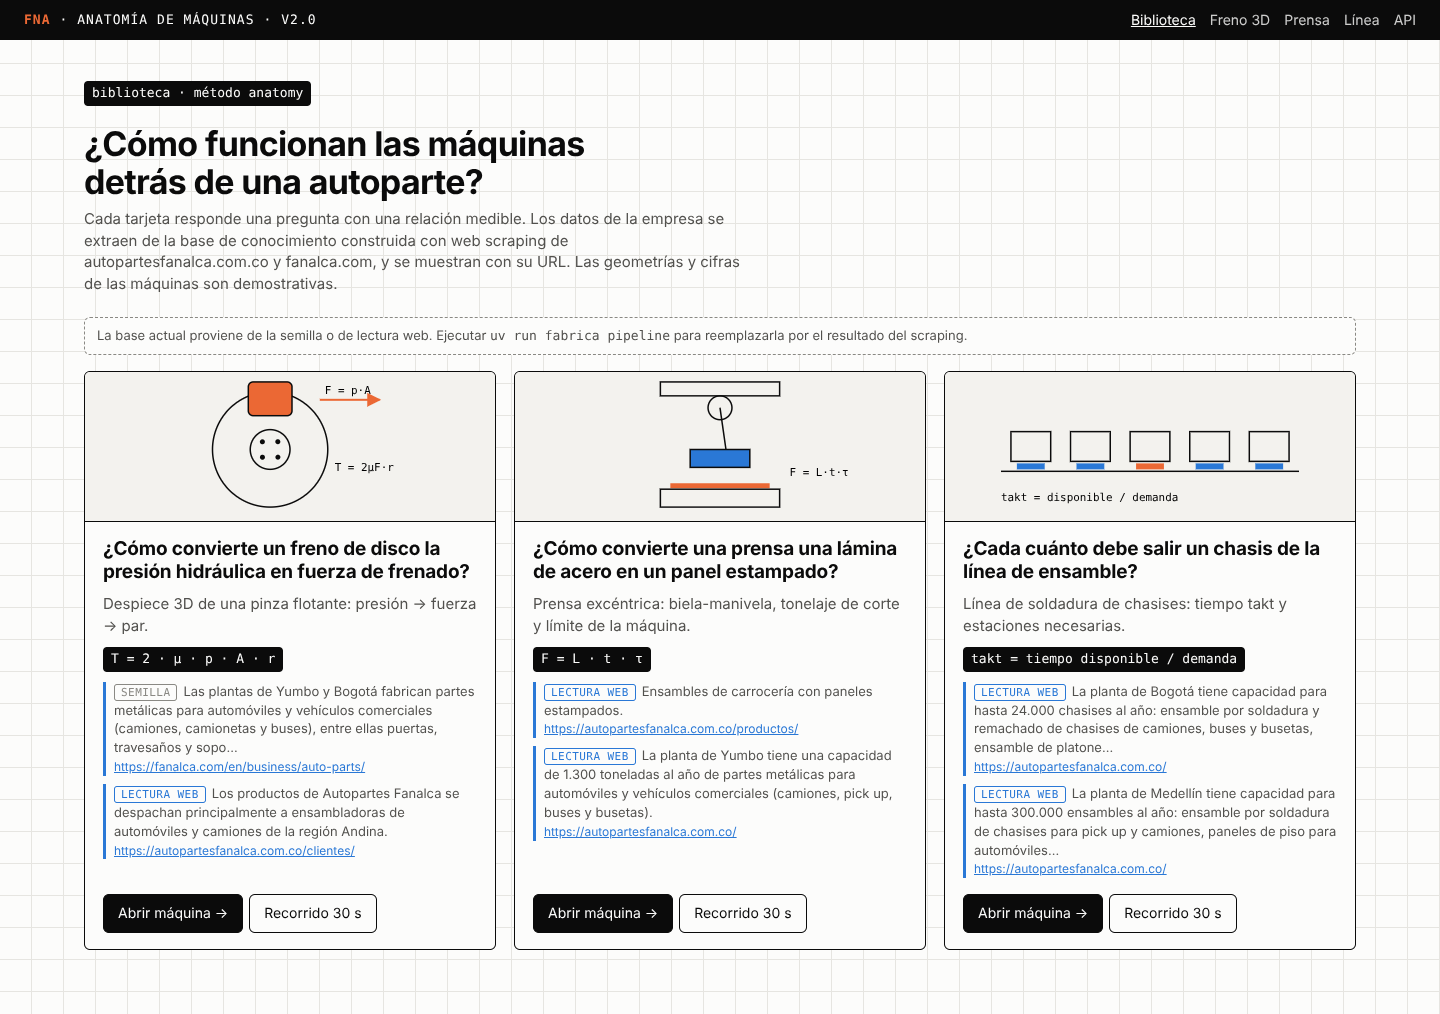
\includegraphics[width=\linewidth,trim=0 0 0 0,clip]{../capturas/v2/01_biblioteca.png}}{\fbox{Captura no disponible}}
\caption{Biblioteca: pregunta como título, una línea, relación, datos de empresa con URL y botones}\label{fig:v2-biblioteca}
\end{figure}

\section{Método Anatomy aplicado}
El método se toma de la skill pública Anatomy, instalada de forma global para Claude Code con
\cmd{npx skills add wheresryan22/anatomy -g -a claude-code} e invocada con \cmd{/anatomy}. Antes de su uso se
revisa su \texttt{SKILL.md}, porque una skill de terceros puede proponer comandos. La skill del proyecto
\texttt{fna-maquinas-anatomia} adapta el método a las reglas de procedencia del sistema.

\begin{table}[H]\centering\small
\caption{Pasos del método y su implementación}\label{tab:anatomia-pasos}
\begin{tabularx}{\linewidth}{@{}P{4.0cm} X@{}}\toprule
Paso & Implementación en el proyecto\\\midrule
1. Instalar la skill & Comando anterior; revisión previa del contenido.\\
2. Elegir una pregunta & Una pregunta por máquina, usada como título de la tarjeta.\\
3. Lógica primero & \ruta{web/src/modelos/*.ts} con pruebas Vitest antes de la escena.\\
4. Legibilidad & 2--4 controles del mecanismo, correr/pausar/reiniciar, cámara lenta, cifras junto a las piezas, pasos numerados e idea principal.\\
5. Estilo & Cuaderno técnico: fondo claro con retícula, tinta, cifras monoespaciadas; naranja = fuerza, azul = movimiento, aqua = estado correcto.\\
6. Revisión crítica & Lista de verificación desplegable en cada máquina.\\
7. Recorrido automático & \texttt{?tour=1}: guion de menos de 30\,s con narración; grabación MP4 con Playwright y FFmpeg.\\
8. Construcción en paralelo & Las tres máquinas comparten \ruta{web/src/componentes/anatomia.tsx}.\\
9. Biblioteca y modo experimento & Tarjetas en \texttt{\#/}; en cada máquina, predicción, ejecución y comparación.\\\bottomrule
\end{tabularx}
\end{table}

\section{Máquinas}
\begin{table}[H]\centering\small
\caption{Máquinas de la biblioteca}\label{tab:anatomia-maquinas}
\begin{tabularx}{\linewidth}{@{}P{2.4cm} X P{2.6cm} P{3.6cm}@{}}\toprule
Máquina & Pregunta & Relación & Controles\\\midrule
Freno de disco (3D) & ¿Cómo convierte un freno de disco la presión hidráulica en fuerza de frenado? & $T = 2\mu pAr$ & presión, $\mu$, velocidad, despiece\\
Prensa de estampado (2D) & ¿Cómo convierte una prensa una lámina de acero en un panel estampado? & $F = L\,t\,\tau$ & espesor, perímetro, material\\
Línea de ensamble (2D) & ¿Cada cuánto debe salir un chasis de la línea de ensamble? & takt = disponible / demanda & demanda, contenido de trabajo, estaciones, turnos\\\bottomrule
\end{tabularx}
\end{table}

\subsection{Prensa de estampado}
La prensa excéntrica combina la cinemática biela-manivela,
\[ s(\theta) = r(1-\cos\theta) + l - \sqrt{l^2 - r^2\sin^2\theta}, \]
con la fuerza de corte $F = L\,t\,\tau$. Si la fuerza supera la capacidad (200\,t, demostrativa), el carro se
detiene al tocar la lámina y la escena muestra la sobrecarga. Los valores de $\tau$ (280, 400 y 450\,MPa) son
rangos típicos publicados para aceros de embutición, estructurales y de alta resistencia; no son especificaciones
de Fanalca. Los datos de empresa provienen de la planta de Yumbo (1\,300\,t/año de partes metálicas) y de la
línea de productos con paneles estampados.

\subsection{Línea de ensamble de chasises}
El takt es el tiempo disponible dividido por la demanda; las estaciones mínimas son
$N = \lceil \text{contenido}/\text{takt}\rceil$ y el ciclo por estación con balanceo ideal es
$c = \text{contenido}/N_{\text{estaciones}}$. Con 24\,000 chasises/año, 288 días, 2 turnos de 8\,h, 240\,min de
contenido y 22 estaciones: takt = 11,52\,min, $N = 21$ y $c = 10{,}91$\,min, por lo que la línea cumple; con
30\,000 chasises/año el takt baja a 9,22\,min, se requieren 27 estaciones y la cola crece.

\begin{figure}[H]\centering
\IfFileExists{../capturas/v2/06_prensa.png}{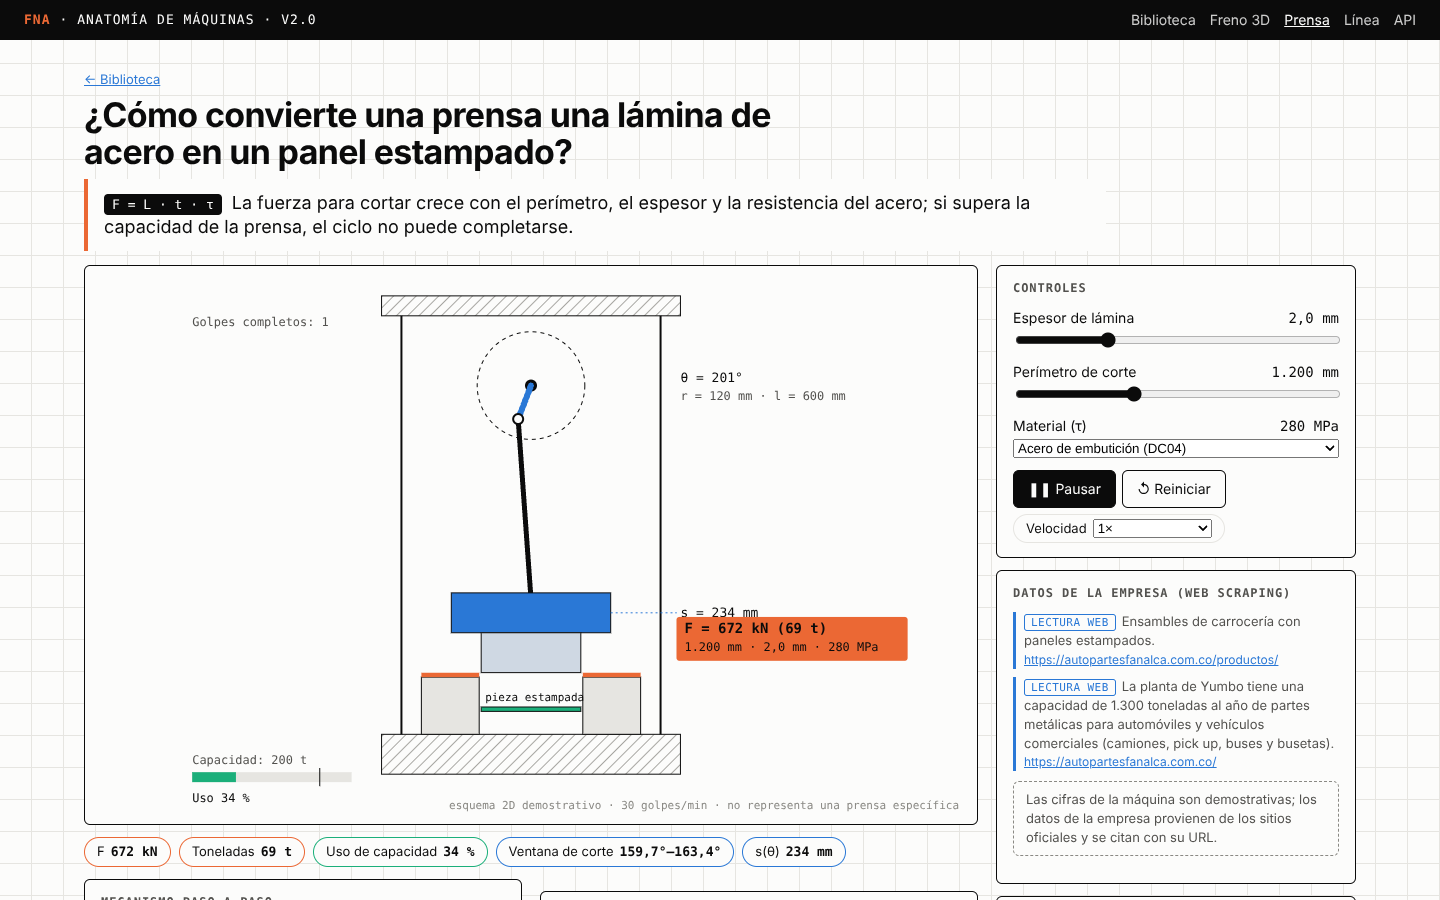
\includegraphics[width=0.49\linewidth]{../capturas/v2/06_prensa.png}}{}\hfill
\IfFileExists{../capturas/v2/07_linea.png}{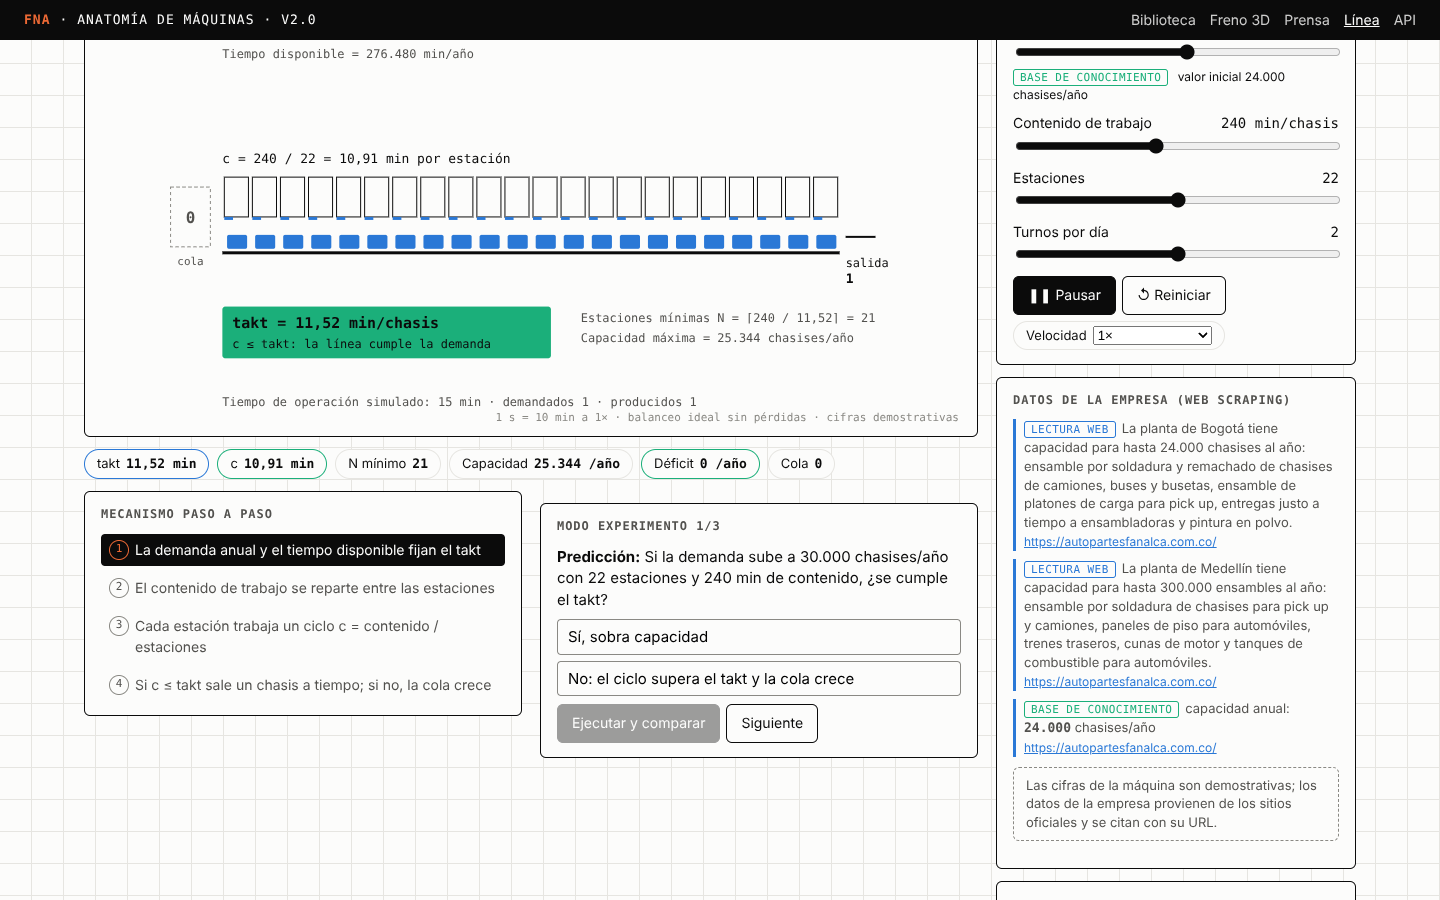
\includegraphics[width=0.49\linewidth]{../capturas/v2/07_linea.png}}{}
\caption{Prensa de estampado (izquierda) y línea de ensamble (derecha)}\label{fig:v2-maquinas2d}
\end{figure}

\section{Modo experimento}
Cada máquina propone predicciones verificables. El usuario elige una opción, la máquina aplica los parámetros y
ejecuta la simulación, y se compara la predicción con el resultado calculado.
\begin{table}[H]\centering\small
\caption{Experimentos incluidos}\label{tab:anatomia-experimentos}
\begin{tabularx}{\linewidth}{@{}P{2.2cm} X P{4.6cm}@{}}\toprule
Máquina & Predicción & Resultado\\\midrule
Freno & Presión de 25 a 50\,bar & El par se duplica; la rueda se bloquea (sin ABS).\\
Freno & $\mu$ de 0,40 a 0,30 & La distancia aumenta alrededor de un tercio ($d \propto 1/\mu$).\\
Freno & Velocidad de 60 a 120\,km/h & La distancia se cuadruplica ($d = v^2/2a$).\\
Prensa & Espesor de 2 a 4\,mm & La fuerza se duplica.\\
Prensa & HSLA de 4\,mm, 1\,200\,mm & 220\,t $>$ 200\,t: el ciclo no se completa.\\
Prensa & Velocidad mínima del carro & En los puntos muertos ($ds/d\theta = 0$).\\
Línea & 30\,000 chasises/año con 22 estaciones & No cumple: el ciclo supera el takt.\\
Línea & Estaciones mínimas para 30\,000 & 27.\\
Línea & De 2 a 3 turnos & El takt aumenta 50\,\%.\\\bottomrule
\end{tabularx}
\end{table}

\section{Recorridos automáticos y videos}
Cada máquina acepta \texttt{?tour=1}: un guion de pasos con tiempos fijos (29\,s el freno, 28\,s la prensa y
26\,s la línea) que cambia parámetros, modos y selección mientras una banda inferior narra el paso. La prueba
\ruta{web/e2e/recorrido.spec.ts} espera la señal de fin, verifica que dure menos de 30\,s, captura los fotogramas
con el \emph{screencast} de Chrome y los codifica en H.264 con FFmpeg en \ruta{docs/videos/}.
\begin{lstlisting}[style=ps]
cd web
npx playwright test --project=recorrido   # docs/videos/recorrido_freno.mp4, _prensa.mp4, _linea.mp4
\end{lstlisting}

\section{Garantías de procedencia}
\begin{itemize}
  \item Ningún texto de empresa se redacta en el frontend: todo proviene de la API con su URL.
  \item Las insignias distinguen \texttt{scraping}, \texttt{lectura web}, \texttt{semilla},
        \texttt{base de conocimiento} y \texttt{demostrativo}.
  \item Las láminas de las tarjetas son esquemas propios y no reproducen productos reales.
  \item La biblioteca advierte cuando la base no proviene del scraping y muestra el comando para regenerarla.
\end{itemize}
